% !TeX spellcheck = en_GB
\documentclass[11pt,a4paper]{article}

\usepackage{fontspec}

\usepackage[english]{babel}
\usepackage[table,xcdraw, svgnames]{xcolor}
\usepackage[margin=3cm, includefoot]{geometry}
\usepackage{graphicx}
\usepackage{subcaption}
\usepackage{float}

\usepackage{ragged2e}
\usepackage{hhline}
%\usepackage{courier}

% Set fonts
\setmainfont{Noto Sans}[BoldFont=Noto Sans Bold, ItalicFont=Noto Sans Italic]
\setmonofont{Noto Sans Mono}[BoldFont=Noto Sans Mono Bold, ItalicFont=Noto Sans Italic]
\setsansfont{Noto Sans}

% To display code
\usepackage{minted}
\usepackage{tcolorbox}
\usepackage{etoolbox}

\usepackage{hyperref}
\hypersetup{
	colorlinks,
	citecolor={black},
	filecolor={black},
	linkcolor={black},
	urlcolor={black},
	pdfauthor={Alireza Beheshti, Rufus Fraanje, Wouter van Velzen},
	pdftitle={Manual Mecabot X},
	pdfsubject={Manual Mecabot X},
	pdfkeywords={manual, Mecabot X},
}

\usepackage{csquotes}

\usepackage{vhistory}

% Used for highlight colors
\usepackage{luacolor}
\usepackage{lua-ul}

% References
\usepackage[backend=biber, style=ieee]{biblatex}
\addbibresource{references.bib}

\begin{document}

% !TeX spellcheck = en_GB
\begin{titlepage}
	\begin{figure}[H]
		\begin{subfigure}{0.5\textwidth}
			\includegraphics[width=.4\textwidth]{pictures/hhs_en_grijs_hex.png}
		\end{subfigure}
		\begin{subfigure}{0.5\textwidth}
			\flushright
			\includegraphics[width=.4\textwidth]{pictures/lectoraat.jpg}
		\end{subfigure}

	\end{figure}
	\vspace{0.5cm}
	\begin{center}
		\Huge{\bfseries MANUAL Mecabot X}\\
		\vspace{-0.75cm}
		\noindent\rule{10cm}{0.4pt}\\
		\Large Connection and Operation guide \\
		%TODO: Add a current picture of the Mecabot X
		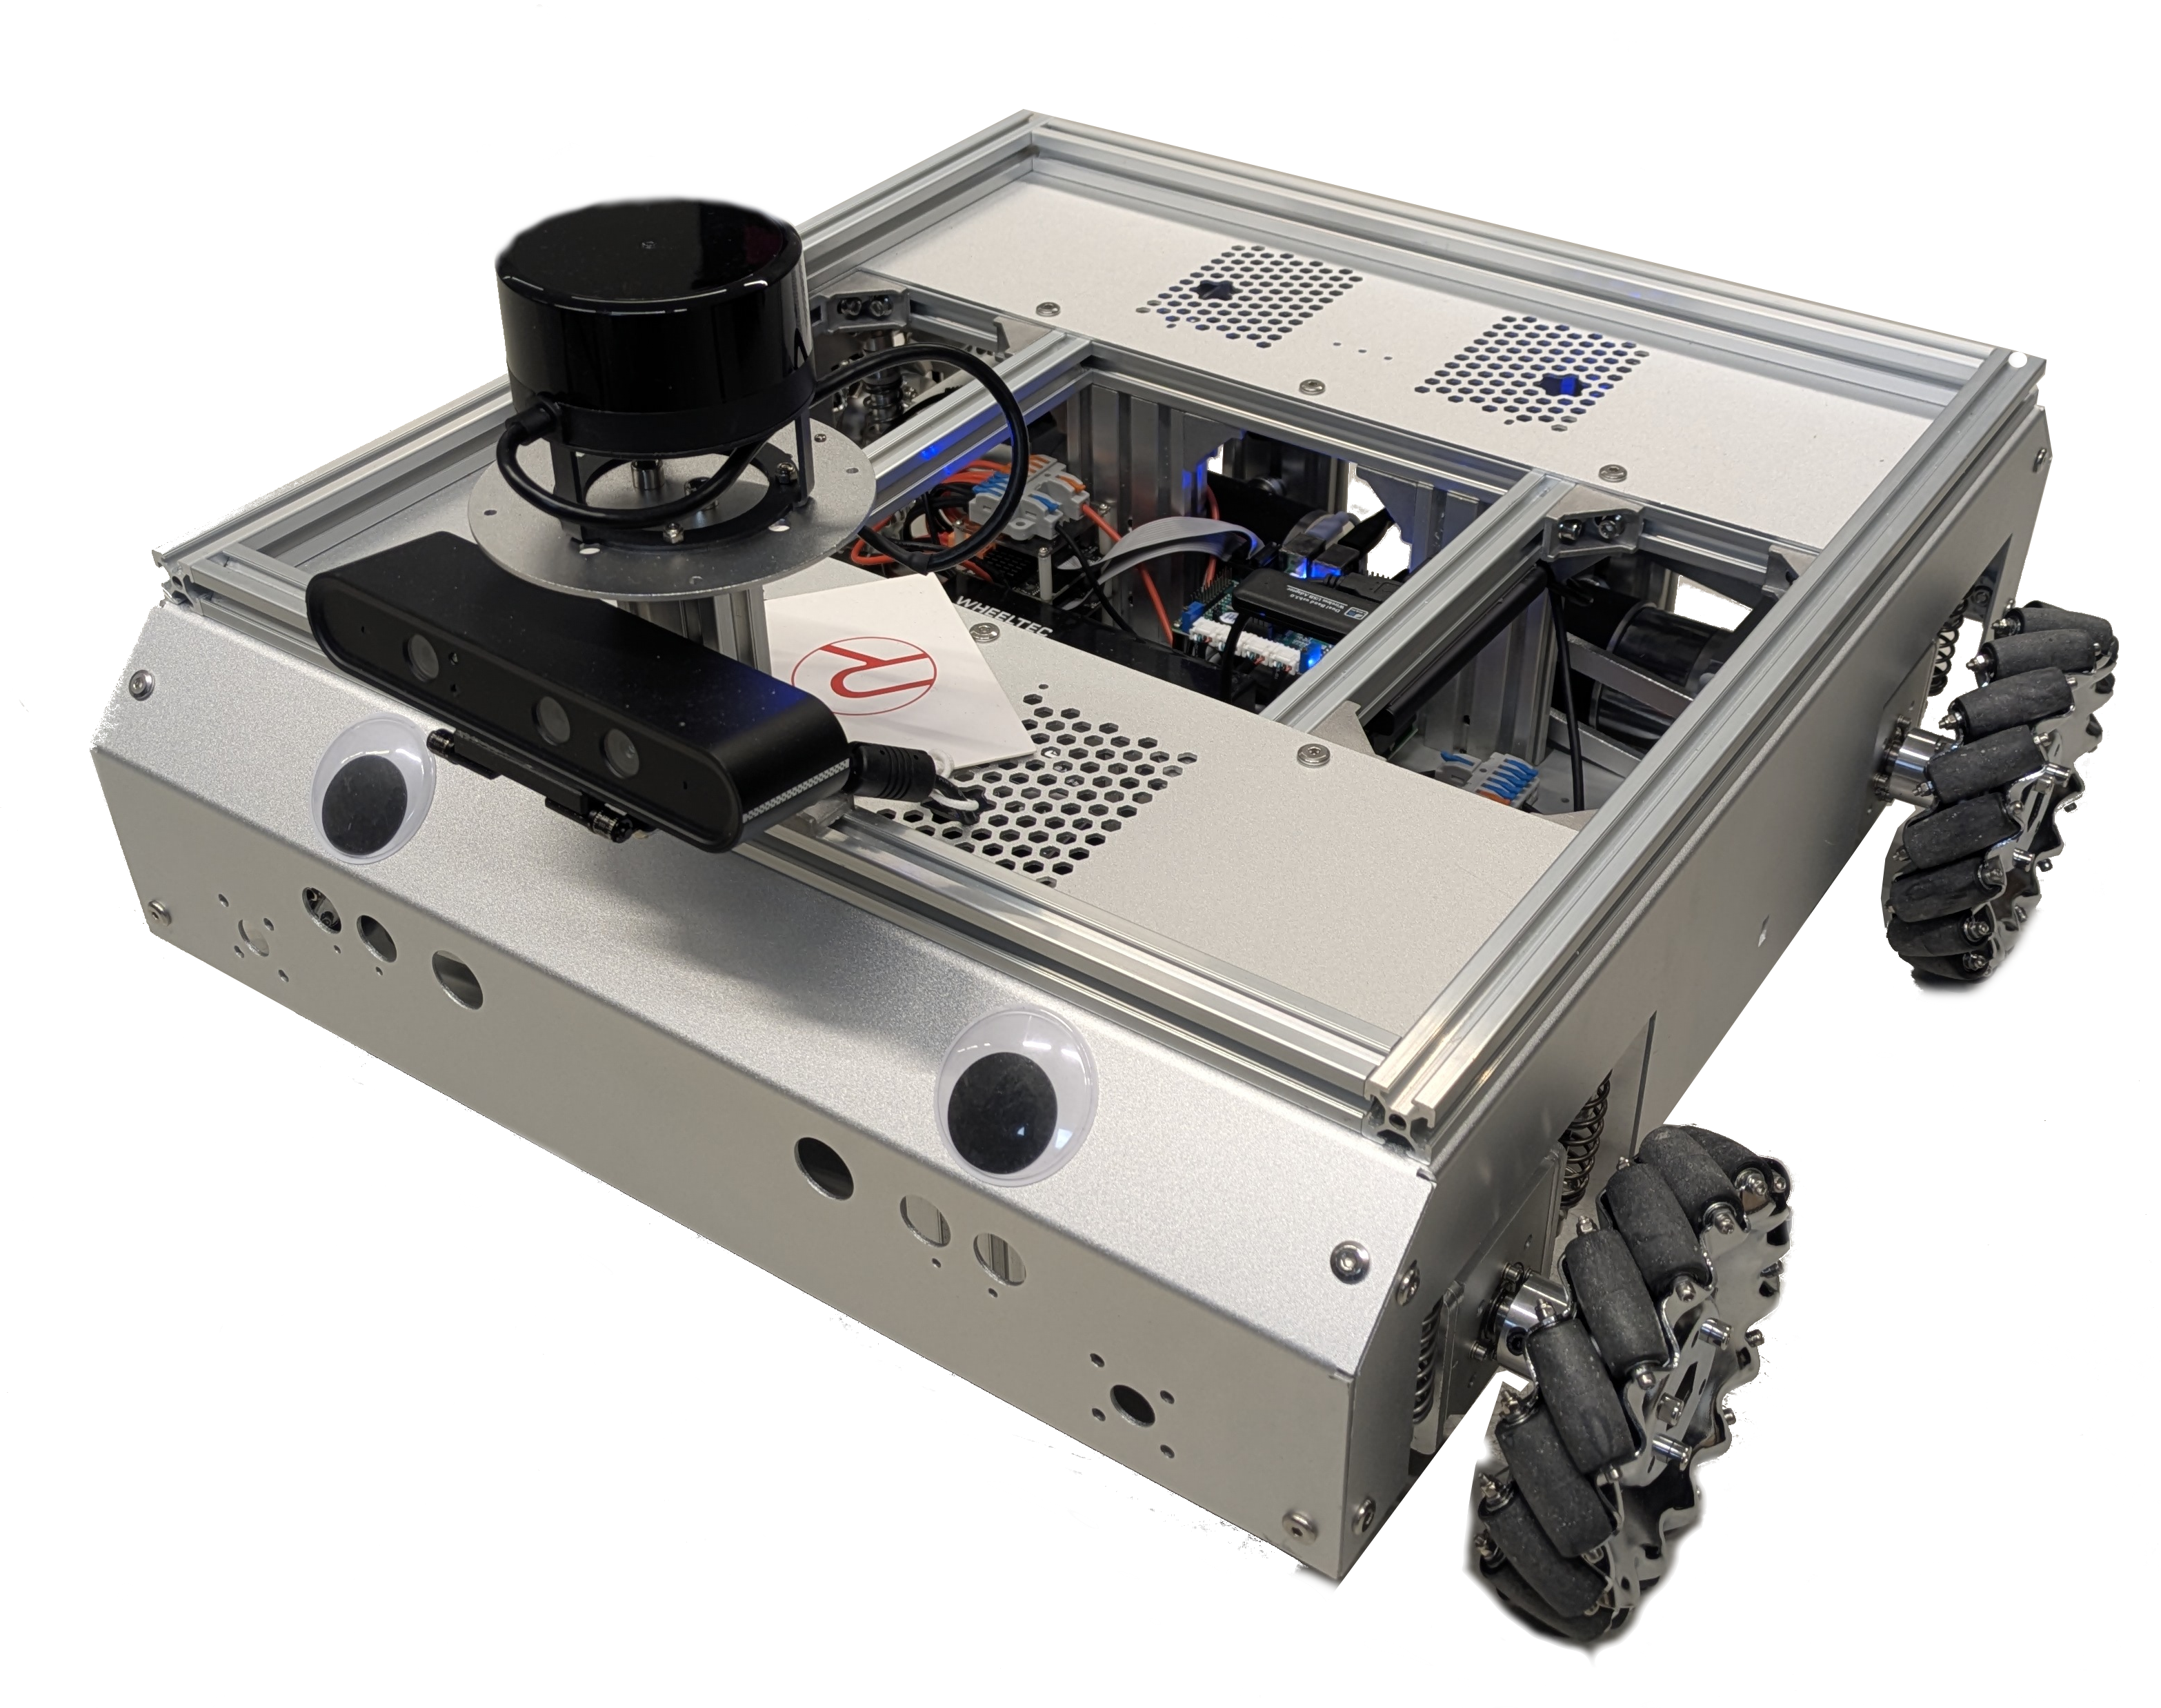
\includegraphics[scale=0.4]{pictures/mecabot_X.png}
	\end{center}

	\begin{flushright}
		{\bfseries Authors:}\\
		Rufus Fraanje \\
		Alireza Behshti \\
		Wouter van Velzen\\

		Jan 2026


	\end{flushright}
	
\begin{versionhistory}
	\vhEntry{1.0}{24.12.01}{Rufus Fraanje| Alireza Beheshti}{Initial release}
	\vhEntry{2.0}{25.12.31}{Wouter van Velzen}{Added more chapters and troubleshooting steps}
\end{versionhistory}
\end{titlepage}


%TODO: Add revision tab

\renewcommand\thesection{}
\setcounter{page}{1}
\pagenumbering{Roman}

\tableofcontents

\newpage

\setcounter{section}{0}
\pagenumbering{arabic}
\renewcommand\thesection{\arabic{section}}

\section{Setup}

This section will go through what is needed to get ROS2 working on your pc. For this section you need a working version of Ubuntu 22.04 and ROS2 installed. Append \ref{sec:appendix_setup} shows how to install ROS2 for specific install options.


% !TeX spellcheck = en_GB
\section{ROS domain ID}

The \texttt{ROS\_DOMAIN\_ID} is a way for multiple ROS 2 nodes to communicate with each other over the network\cite{domain_id}. For example RVIZ2 can communicate with the cartographer program on the Mecabot to visualize the room the robot is in. For ROS 2 nodes to communicate, they must be in the same \texttt{ROS\_DOMAIN\_ID}. This means the laptop and the Mecabot need to be on the same network and the same subnet.

This is possible with a VM or WSL, but difficult. \textbf{Therefore it is recommended to use a PC or laptop with a Linux operating system.}
\newpage

The \texttt{ROS\_DOMAIN\_ID} is an environment variable in ROS 2 that allows you to run multiple ROS 2 processes on the same network without them interfering with each other.

Here are some advantages of using \texttt{ROS\_DOMAIN\_ID}:

\begin{itemize}
	\item \textbf{Isolation:} By setting different \texttt{ROS\_DOMAIN\_ID} values, you can isolate different sets of nodes from each other. This is useful when you have multiple robots or systems on the same network and want to ensure they don't interfere with each other.
	\item \textbf{Scalability:} It makes it easier to scale your system by adding more nodes or robots without worrying about conflicts. Each group of nodes can operate independently within its own domain.
	\item \textbf{Simplified configuration:} It simplifies the configuration of your network by allowing you to manage communication between specific groups of nodes more easily.
	\item \textbf{Enhanced security:} By isolating different parts of your system, you can enhance security by limiting communication to only the necessary nodes within a domain.
	\item Using \texttt{ROS\_DOMAIN\_ID} can greatly improve the organization and efficiency of your ROS 2 setup, especially in complex environments with multiple robots or systems.
\end{itemize}

\subsection{Setup ROS domain ID}

The following is needed to setup the \texttt{ROS\_DOMAIN\_ID} on your laptop and on the Mecabot X. In this chapter you need to open multiple terminals. These terminals are for the laptop and for the Mecabot. If a command needs to be run on the laptop the ''script box'' will be \colorbox{Gainsboro}{grey}. If it needs to be run on the Mecabot the ''script box'' will be \colorbox{NavajoWhite}{yellow}.

%TODO: set the correct collor in the text.

\subsubsection*{Connect the Laptop to the network}
Make sure the laptop and the Mecabot are connected on the same network. If you don't know how you can check chapter \ref{sec:setup}.

\subsubsection*{Set the ROS domain ID}
The \texttt{ROS\_DOMAIN\_ID} functions as a communication channel between the laptop and the robot. It is essential that both devices are configure to operate on the same channel.

\paragraph{On laptop:}
\begin{itemize}
	\item Open a terminal.
	\item Run these commands:
\end{itemize}

\begin{tcolorbox}[colback=Gainsboro]
\begin{minted}{bash}
source /opt/ros/humble/setup.bash
export ROS_DOMAIN_ID=10
\end{minted}
\end{tcolorbox}

\textbf{NOTE: If ''\texttt{source /opt/ros/humble/setup.bash}'' doesn't work, it might mean you haven't installed ROS proparly. Check appendix \ref{sec:appendix_setup} for more info.}

\paragraph{On Mecabot:}
\begin{itemize}
	\item Open a terminal.
	\item Run these commands:
\end{itemize}

\begin{tcolorbox}[colback=NavajoWhite]
\begin{minted}{bash}
source /opt/ros/humble/setup.bash
export ROS_DOMAIN_ID=10
\end{minted}
\end{tcolorbox}

\subsubsection*{Verify connectivity}
When the \texttt{ROS\_DOMAIN\_ID} is set on both the laptop and the Mecabot we can verify the connection. This can be done using the following command

\begin{tcolorbox}[colback=Gainsboro]
\begin{minted}{bash}
ping 192.168.0.100
\end{minted}
\end{tcolorbox}

\textbf{NOTE: Should be the IP that you found in chapter \ref{sec:setup}.}

If the Mecabot doesn't respond to the ping request, there is something wrong with the network connection between your laptop and the Mecabot.

\subsubsection*{Run ROS Nodes}

ROS 2 comes with a simple test program to test the connectivity between different devices on the same \texttt{ROS\_DOMAIN\_ID}. To test this run the following commands.

\paragraph{On Laptop:}
\begin{itemize}
	\item Use existing terminal.
	\item Run the following command:
\end{itemize}

\begin{tcolorbox}[colback=Gainsboro]
\begin{minted}{bash}
ros2 run demo_nodes_cpp talker
\end{minted}
\end{tcolorbox}

\textbf{NOTE: If the ros2 command isn't found or the ''\texttt{demo\_nodes\_cpp}'' then the previous ''\texttt{source /opt/ros/humble/setup.bash}'' didn't work. Go to appendix \ref{sec:appendix_setup} for more info.}

\paragraph{On Mecabot:}

\begin{itemize}
	\item Use existing terminal.
	\item Run the following command:
\end{itemize}

\begin{tcolorbox}[colback=NavajoWhite]
\begin{minted}{bash}
ros2 run demo_nodes_cpp listener
\end{minted}
\end{tcolorbox}

If the robot and the laptop are correctly put on the same \texttt{ROS\_DOMAIN\_ID} the you should see the following in the terminal. \textbf{TODO: Make picture of the terminal whil running this script.}
%TODO: add figure for the correct ouput.

\newpage


% !TeX spellcheck = en_GB
\section{Controlling the Mecabot}
The Mecabot can be manually controlled using multiple different methods. In this chapter the known connection methods are explained.

\subsection{Controlling the Mecabot with a PS2 controller}
The Mecabot can be operated using a PS2 controller. Follow these steps to set up and utilize the PS2 controller for robot control.

This is the easiest way to control the Mecabot. 

\subsubsection*{Connect the controller}

\begin{itemize}
	\item Plug in the PS2 controller to the Mecabot X.
	\item Wait until the indicator light on the controller turn red, indicating a successful connection.
	\begin{itemize}
		\item Sometimes you need to press the ''Analog'' button on the controller.
	\end{itemize}
\end{itemize}

\begin{figure}[H]
	\centering
	\includegraphics[width=0.5\linewidth]{./pictures/PS2_controller.jpg}
	\caption{PS2 controller connection}
	\label{fig:PS2_controller}
\end{figure}

\subsubsection*{Activate the controller}

\begin{itemize}
	\item Press the start button on the PS2 controller to activate it.
\end{itemize}

\subsubsection*{Switch to PS2 control mode}

\begin{itemize}
	\item Look at the screen on the PCB board of the Mecabot X.
	\item Push the left joystick forward to switch the control mode from ROS to PS2. The screen will display the current control mode, confirming the change (see figure \ref{fig:PS2_oled} for visual guidance).
\end{itemize}

\begin{figure}[H]
	\centering
	\includegraphics[width=0.5\linewidth]{./pictures/PS2_oled.jpg}
	\caption{Switch to PS2 control mode}
	\label{fig:PS2_oled}
\end{figure}

\subsubsection*{PS2 controller controls}
\begin{itemize}
	\item \textbf{Left joystick}: Controls translation movement (forward, backwards, left, right).
	\item \textbf{Right joystick}: Controls rotation movement (turning the robot).
	\item \textbf{L1 button}: Increases the robot's speed (acceleration).
	\item \textbf{L2 button}: Decrease the robot's speed (deceleration).
\end{itemize}


\subsection{Controlling the Mecabot with ROS 2}

In this chapter, we will discuss how to set up the Mecabot to control it using your laptops keyboard. It assumes you've followed the steps of the previous chapters before continuing.

Open an terminal and connect to the Mecabot. Run the following commands:

\begin{tcolorbox}[colback=NavajoWhite]
\begin{minted}{bash}
source ~/wheeltec_ros2/install/setup.bash
ros2 launch turn_on_wheeltec_robot turn_on_wheeltec_robot.launch.py
\end{minted}
\end{tcolorbox}

This will enable the sensors en motor of the Mecabot.\\
\textbf{NOTE: a lot of the commands in the future of the document do this for you in the background. If you run this command in parallel, it could crash the system.}

Open an second terminal and also connect this to the Mecabot. Run the following command in this second terminal:

\begin{tcolorbox}[colback=NavajoWhite]
\begin{minted}{bash}
source ~/wheeltec_ros2/install/setup.bash
ros2 run wheeltec_robot_keyboard wheeltec_keyboard
\end{minted}
\end{tcolorbox}

Figure \ref{fig:wheeltec_keyboard} shows how your terminal should look like.

\begin{figure}[H]
	\centering
	\includegraphics[width=0.6\linewidth]{./pictures/wheeltec_keyboard.png}
	\caption{Wheeltec keyboard command}
	\label{fig:wheeltec_keyboard}
\end{figure}

\subsection{Controlling the Mecabot with a joystick controller}
The Mecabot can also be controlled using a wireless joystick controller. Follow the following steps to set up and utilize the joystick controller for robot control:

\begin{itemize}
	\item Connect the joystick's dongle in one of the usb ports on the Mecabot X.
	\begin{itemize}
		\item Dongle is usually already connected in the robot.
	\end{itemize}
	\item turn on the joystick.
	\item Connect to the Mecabot using SSH and run the following command:
\end{itemize}

\begin{tcolorbox}[colback=NavajoWhite]
\begin{minted}{bash}
ros2 launch wheeltec_joy wheeltec_joy.launch.py
\end{minted}
\end{tcolorbox}

This will execute the script and enable control of the Mecabot X using the joystick.


\newpage

% !TeX spellcheck = en_GB
\section{Creating a map}\label{sec:create_map}
For the Mecabot X to travel autonomously it needs a map. This can be done in three steps.
\begin{itemize}
	\item Start up cartographer.
	\item Drive around (creating the map).
	\item Save the map.
\end{itemize}

Cartographer is a program that is created by the Roboworks team. It uses SLAM to map it's surroundings. In robotics, SLAM is the term given to \textbf{S}imultaneous \textbf{L}ocalization \textbf{a}nd \textbf{M}apping algorithms\cite{slam_toolbox, slam_wiki}. As the name suggests, this allows the robot to build a map of an unknown environment, as well as improving the map with new features over time. Localization refers to the robot determining its position in relation to the map, termed the global frame. This can be compared to a submarine using its radar sensor to continuously map the terrain of the ocean.

This chapter assumes you can already connect to the robot and have setup a ''\texttt{ROS\_DOMAIN\_ID}''. If not look into chapter \ref{sec:setup} and \ref{sec:ROS_ID}.

If a command needs to be run on the laptop the ''script box'' will be \colorbox{Gainsboro}{grey}. If it needs to be run on the Mecabot the ''script box'' will be \colorbox{NavajoWhite}{yellow}.

\subsection{Start cartographer}

Run the following command on the Mecabot to start up cartographer.

\begin{tcolorbox}[colback=NavajoWhite]
	\begin{minted}{bash}
source ~/wheeltec_ros2/install/setup.bash
ros2 launch wheeltec_cartographer cartographer.launch.py
\end{minted}
\end{tcolorbox}

\textbf{Note: this will start the LiDAR without blind spots. If you want to start with blind spots, replace: ''\texttt{cartographer.launch.py}'' with: ''\texttt{cartographer\_w\_blindspots.launch.py}''.}

Next you can open RVIZ on your laptop to see the live cartographer data.

\begin{tcolorbox}[colback=Gainsboro]
	\begin{minted}{bash}
ros2 launch wheeltec_rviz2 wheeltec_rviz.launch.py
\end{minted}
\end{tcolorbox}

Figure \ref{fig:RVIZ_Cartographer} shows the current map in RVIZ.

\begin{figure}[H]
	\centering
	\includegraphics[width=0.9\linewidth]{./pictures/RVIZ_cartographer.png}
	\caption{Cartographer on RVIZ2}
	\label{fig:RVIZ_Cartographer}
\end{figure}

\subsection{Driving around}

By utilizing one of the movement packages, (see chapter \ref{sec:controlling}) the operator can navigate the robot and illuminate the surrounding map. Using the wired controller is the easiest way.

The map being visualized can take some time so move slowly. (going sideways is inaccurate. Try avoid this movement.)

\subsection{Saving the map}

When done creating the map, you can save the map. This map can be used by nav2 to to drive autonomously. Open a new terminal (on the Mecabot) and type the following command:

\begin{tcolorbox}[colback=NavajoWhite]
	\begin{minted}{bash}
ros2 run nav2_map_server map_saver_cli -f <directory path>
\end{minted}
\end{tcolorbox}

This command initiates the execution of a ROS2 node, nav2\_map\_server specifies the package containing the node, and map\_saver\_cli is the node responsible for saving the map\cite{nav2_saver}. The ''\texttt{-f}'' flag followed by \texttt{<directory path>} indicates the file path where the map should be saved. For example, to save the map to a directory named maps in the home directory, \texttt{<directory path>} would be replace with: ''\texttt{\~{}/maps/my\_map}''.

Figure \ref{fig:map_saver_succes} shows the output of the map being saved.

\begin{figure}[H]
	\centering
	\includegraphics[width=0.9\linewidth]{./pictures/map_saver_correct.png}
	\caption{Successfully saved map}
	\label{fig:map_saver_succes}
\end{figure}

\subsection{Troubleshooting}

\subsubsection{Cartographer command is not found}

Is your ROS environment sourced?

\begin{tcolorbox}[colback=NavajoWhite]
	\begin{minted}{bash}
source ~/wheeltec_ros2/install/setup.bash
\end{minted}
\end{tcolorbox}

\subsubsection{Cartographer is not working}

\paragraph{Check LiDAR}
Check LiDAR is functional.

% ros2 launch turn_on_wheeltec_robot wheeltec_lidar.launch.py

\begin{tcolorbox}[colback=NavajoWhite]
	\begin{minted}{bash}
ros2 launch turn_on_wheeltec_robot wheeltec_lidar.launch.py
	\end{minted}
\end{tcolorbox}

\paragraph{Terminal hangs}
Terminal shows the following message: ''\texttt{Waiting for robot\_description to be published on the robot\_description topic...}'' and no new text.

Sometimes cartographer doesn't start correctly. retry starting the program. If that doesn't work reboot the robot using the following command:

\begin{tcolorbox}[colback=NavajoWhite]
	\begin{minted}{bash}
sudo shutdown -r now
	\end{minted}
\end{tcolorbox}


\subsubsection{NO RVIZ data}

Does your laptop and the Mecabot have the same ''\texttt{ROS\_DOMAIN\_ID}''?

\begin{tcolorbox}[colback=Gainsboro]
\begin{minted}{bash}
export ROS_DOMAIN_ID=10
\end{minted}
\end{tcolorbox}

Check if the simple ROS demo\_node\_cpp talker and listener is working. (See chapter \ref{sec:ROS_ID}.)

If the talker and listener aren't working your laptop and the Mecabot are not on the same network. (Using WSL or a VM.)

Advise: use Linux natively.

\subsubsection{Can't save map}

Does your new terminal have the same ''\texttt{ROS\_DOMAIN\_ID}'' as the cartographer?

\paragraph{Error message}

sometimes saving the map gives the following error message: ''\textcolor{Red}{Failed to spin map subscription}''. Figure \ref{fig:map_saver_fail} shows the failed output. This error has multiple solutions.

The ''\texttt{-f}'' tag doesn't always work. Try a different directory or name or remove the tag all together. If no tag is given the program will save with a random name in the current directory. 

Sometimes there is no reason. If you retry it again without doing anything different it just works.

\begin{figure}[H]
	\centering
	\includegraphics[width=0.9\linewidth]{./pictures/map_saver_incorrect.png}
	\caption{Failed saved map}
	\label{fig:map_saver_fail}
\end{figure}

\newpage


% !TeX spellcheck = en_GB
\section{Autonomous driving}\label{sec:autonomous}

This chapter shows an example on how to make the robot drive autonomously through an environment. For this to work you'll need an saved map as explained in the previous chapter.

\subsection{Trouble shooting}

\subsubsection{NO RVIZ data}

Does your laptop and the Mecabot have the same ''\texttt{ROS\_DOMAIN\_ID}''?

\begin{tcolorbox}[colback=Gainsboro]
	\begin{minted}{bash}
export ROS_DOMAIN_ID=10
	\end{minted}
\end{tcolorbox}

Check if the simple ROS demo\_node\_cpp talker and listener is working. (See chapter \ref{sec:ROS_ID}.)

If the talker and listener aren't working your laptop and the Mecabot are not on the same network. (Using WSL or a VM.)

Advise: use Linux natively.

\subsubsection{RVIZ is showing the wrong map}


Navigation 2 info.

\newpage

% !TeX spellcheck = en_GB
\section{Mecabot drive autonomously}

\subsection{Creating the map}

Info to create a map of the place where to autonomously drive.


\subsection{Save the map}

Info how (and where) to save the map created

\subsection{Set waypoints}

How to create waypoints and set them to create a route.

\subsection{Activate nav 2}

How to activate NAV 2 to autonomously drive around.

\newpage

% !TeX spellcheck = en_GB
\section{Commands}\label{sec:commands}
Bellow are the ros2 commands that are shipped with the standard package. It shows what the commands do and how they work.

To run commands on PC you need to download the needed binary's. Appendix \ref{sec:appendix_copy_bin} tells you how to download the binary from the Mecabot X. Appendix \ref{sec:appendix_compile} show how to compile the binary's yourself.

 If a command needs to be run on the laptop the ''script box'' will be \colorbox{Gainsboro}{grey}. If it needs to be run on the Mecabot the ''script box'' will be \colorbox{NavajoWhite}{yellow}.

\subsection{wheeltec\_rviz2}\label{sec:rviz}

RVIZ2 is an acronym for ROS Visualization 2\cite{RVIZ2}. It is a sophisticated visualization tool developed for ROS 2. It offers a graphical interface that enables users to visualize various aspects of a robot's state, including sensor data, the robot's position, and its planned navigation path.

RVIZ2 should be run on a laptop that is connected to the same \texttt{ROS\_DOMAIN\_ID} and on the same network as the Mecabot.

Run the following command on your laptop:

\begin{tcolorbox}[colback=Gainsboro]
\begin{minted}{bash}
source ~/wheeltec_ros2/install/setup.bash
export ROS_DOMAIN_ID=10
ros2 launch wheeltec_rviz2 wheeltec_rviz.launch.py
\end{minted}
\end{tcolorbox}

This should run a RVIZ window. Figure \ref{fig:RVIZ2} shows an example.

\begin{figure}[H]
	\centering
	\includegraphics[width=0.8\linewidth]{./pictures/RVIZ2.png}
	\caption{Empty RVIZ2 window}
	\label{fig:RVIZ2}
\end{figure}

\subsection{wheeltec\_keyboard}


\subsubsection*{Command}

\begin{tcolorbox}[colback=NavajoWhite]
\begin{minted}{bash}
ros2 run wheeltec_robot_keyboard wheeltec_keyboard
\end{minted}
\end{tcolorbox}

\subsubsection*{Arguments}

None


\subsection{wheeltec\_joy}

\subsubsection*{Command}

\begin{tcolorbox}[colback=NavajoWhite]
\begin{minted}{bash}
ros2 launch wheeltec_joy wheeltec_joy.launch.py
\end{minted}
\end{tcolorbox}

\subsubsection*{Arguments}

None

\subsection{turn\_on\_wheeltec\_robot}
These commands can be used manually. But other commands already do this in the background when booting up.

\subsubsection*{Command}

\begin{tcolorbox}[colback=NavajoWhite]
\begin{minted}{bash}
ros2 launch turn_on_wheletec_robot <ARGUMENT>
\end{minted}
\end{tcolorbox}

\paragraph{Most used:}
The following arguments are most used. The rest of the commands are shown in the arguments section.

Completely turn on the Mecabot.
\begin{tcolorbox}[colback=NavajoWhite]
\begin{minted}{bash}
ros2 launch turn_on_wheletec_robot turn_on_wheeltec_robot.launch.py
\end{minted}
\end{tcolorbox}


Turns on the LiDAR:
\begin{tcolorbox}[colback=NavajoWhite]
\begin{minted}{bash}
ros2 launch turn_on_wheletec_robot wheeltec_lidar.launch.py
\end{minted}
\end{tcolorbox}

\textbf{Turns on sensors?:}
\begin{tcolorbox}[colback=NavajoWhite]
\begin{minted}{bash}
ros2 launch turn_on_wheletec_robot wheeltec_sensors.launch.py
\end{minted}
\end{tcolorbox}

\subsubsection*{Arguments}

%TODO: Find out what all the arguments do!
\begin{itemize}
	\item ''\texttt{base\_serial.launch.py}''
	\begin{itemize}
		\item \textbf{Start serial port?}
	\end{itemize}
	\item ''\texttt{robot\_mode\_description.launch.py}''
	\begin{itemize}
		\item \textbf{Setup robot description?}
	\end{itemize}
	\item ''\texttt{robot\_mode\_description\_minibot.launch.py}''
	\begin{itemize}
		\item \textbf{Same as ''\texttt{robot\_mode\_description.launch.py}'' but for different type of robot?}
	\end{itemize}
	\item ''\texttt{robotandlidar.launch.py}''
	\begin{itemize}
		\item \textbf{Does the same as ''\texttt{turn\_on\_wheeltec.launch.py}'' robot?}
	\end{itemize}
	\item ''\texttt{turn\_on\_wheeltec\_robot.launch.py}''
	\begin{itemize}
		\item Turns on all the sensors of the Mecabot.
	\end{itemize}
	\item ''\texttt{wheeltec\_camera.launch.py}''
	\begin{itemize}
		\item Turns on the camera unit of the Mecabot.
	\end{itemize}
	\item ''\texttt{wheeltec\_ekf.launch.py}''
	\begin{itemize}
		\item \textbf{Turns on the EKF unit? [what is EKF?]}
	\end{itemize}
\end{itemize}

\subsection{wheeltec\_cartographer}



\subsection{nav2\_map\_saver}

\subsection{wheeltec\_nav2}


\newpage

\addcontentsline{toc}{section}{References}
\printbibliography

%appendix
\newpage
\section{Appendix}\label{sec:appendix}
\renewcommand\thesubsection{\Alph{subsection}}

\subsection{Setup environment}\label{sec:appendix_setup}

\subsubsection{System and software requirement}
The Mecabot X uses ROS Humble to run it's autonomous program. To use ROS2 you need the following specs:

\begin{itemize}
	\item ROS2 version: Humble
	\item OS: Ubuntu 22.04
\end{itemize}

This can be done in three different ways. If you're using Windows you can setup WSL (\ref{sec:appendix_wsl_setup}) or install a VM (\ref{sec:appendix_vm_setup}). If you're dual booting or only using Linux follow appendix \ref{sec:appendix_linux_setup}.

\textbf{NOTE: WSL and VM can't directly communicate with the} \texttt{ROS\_DOMAIN\_ID} \textbf{This mean you can't (easily) visualise what the Mecabot X is doing using these options.}

\subsubsection{WSL setup}\label{sec:appendix_wsl_setup}
WSL stand for Windows subsystem for Linux. It can be used to run Linux software close to native on your Windows PC. This document will use the tutorial create by Microsoft\cite{WinWSL}.

\paragraph{Optional: enable ''sudo'' for Windows}
Sudo for Windows allows you to use the Sudo command like it's used on Linux PC's. This way you don't need to open PowerShell as an administrator.

Go to settings->System->Advanced. There you can enable ''Enable sudo''. See figure \ref{fig:appendix_win_sudo_1} how it looks like.

\begin{figure}[H]
	\centering
	\includegraphics[width=0.7\linewidth]{./pictures/win_sudo_1.png}
	\caption{Windows enable sudo}
	\label{fig:appendix_win_sudo_1}
\end{figure}

\paragraph{Enable WSL}
Go to settings. In the search bar type ''Turn Windows features on or off''. A screen should appear like shown in figure \ref{fig:appendix_windows_features}.

\begin{figure}[H]
	\centering
	\includegraphics[width=0.5\linewidth]{./pictures/Windows_features.png}
	\caption{Windows Features}
	\label{fig:appendix_windows_features}
\end{figure}

Search for the entry labelled ''Windows Subsystem for Linux'' and enable the feature. The system will ask to be rebooted. After the reboot follow the next steps.

After the reboot open Powershell and type the following:

\begin{tcolorbox}
\begin{minted}{bash}
wsl --install
\end{minted}
\end{tcolorbox}

After the command is done you need to reboot the system again.

\paragraph{Install Ubuntu 22.04}
After the reboot open the Microsoft Store and search ''Ubuntu 22.04''. \\
\textbf{It needs to be Ubuntu 22.04 newer version don't work with ROS2 Humble.} \\
Figure \ref{fig:appendix_windows_store} shows how the store looks like.

\begin{figure}[H]
	\centering
	\includegraphics[width=0.5\linewidth]{./pictures/win_download_ubuntu.png}
	\caption{Microsoft Store Ubuntu install}
	\label{fig:appendix_windows_store}
\end{figure}

After the download press the open button. It will ask for the following information:

\begin{itemize}
	\item ''Enter new UNIX username:''
	\begin{itemize}
		\item This is the username for the Linux installation.
	\end{itemize}
	\item ''New password:''
	\begin{itemize}
		\item This is the password for the Linux installation. It won't show the characters even though you're typing.
	\end{itemize}
	\item ''Retype new password:''
	\begin{itemize}
		\item Retype the previously typed password.
	\end{itemize}
\end{itemize}

It should look like shown in figure \ref{fig:appendix_win_wsl_terminal}.

\begin{figure}[H]
	\centering
	\includegraphics[width=0.8\linewidth]{./pictures/win_wsl_terminal.png}
	\caption{WSL terminal setup}
	\label{fig:appendix_win_wsl_terminal}
\end{figure}

After the install you should update the Ubuntu install using the following commands:

\begin{tcolorbox}
\begin{minted}{bash}
sudo apt update
sudo apt upgrade -y
\end{minted}
\end{tcolorbox}

It will ask for the password you just setup.

\paragraph{Setup graphical WSL}
WSL can run graphical Linux applications\cite{WinWSLG}. This is needed to run stuff like RVIZ2. To do this the WSL Ubuntu system needs to be run with WSL 2.

Open Powershell. and run the following command:

\begin{tcolorbox}
\begin{minted}{bash}
wsl -l -v
\end{minted}
\end{tcolorbox}

It should show the following output:

\begin{tcolorbox}[colback=LightGoldenrodYellow]
\begin{minted}{bash}
  NAME            STATE           VERSION
* Ubuntu-22.04    Running         2
\end{minted}
\end{tcolorbox}

If the version is 2 you can continue to \ref{sec:appendix_check_gui} otherwise follow the next commands.

If the state is ''running'' you need to stop the WSL instance. Using the following command:

\begin{tcolorbox}
\begin{minted}{bash}
wsl --shutdown
\end{minted}
\end{tcolorbox}

Check if it's stopped using:

\begin{tcolorbox}
\begin{minted}{bash}
wsl -l -v
\end{minted}
\end{tcolorbox}

the ''\texttt{STATE}'' should be ''Stopped''. After the system is stopped run the following command:

\begin{tcolorbox}
\begin{minted}{bash}
wsl --set-version _distro_name_ 2
\end{minted}
\end{tcolorbox}

The ''\texttt{\_distro\_name\_}'' should be the name you get running ''\texttt{wsl -l -v}''. In this example the name is: ''\texttt{Ubuntu-22.04}''. After hitting enter it will upgrade from WSL 1 to WSL 2. This can take several minutes.

\paragraph{Check GUI}\label{sec:appendix_check_gui}

If you're running WSL2 you can run Graphical Linux applications. Here are some commands to test if this function is working. The following commands need to be run in the WSL ubuntu terminal.

Install gedit:

\begin{tcolorbox}
\begin{minted}{bash}
sudo apt install gedit
\end{minted}
\end{tcolorbox}

After installing run the following command:

\begin{tcolorbox}
\begin{minted}{bash}
gedit
\end{minted}
\end{tcolorbox}

This should run a graphical text editor. Figure \ref{fig:appendix_gedit} shows how the application looks like.

\begin{figure}[H]
	\centering
	\includegraphics[width=0.5\linewidth]{./pictures/win_wsl_gedit.png}
	\caption{Gedit running in WSL}
	\label{fig:appendix_gedit}
\end{figure}

Now you can follow the Linux setup (appendix \ref{sec:appendix_linux_setup}) to install ROS2 in the WSL terminal.

\subsubsection{VM setup}\label{sec:appendix_vm_setup}

\subsubsection{Linux setup}\label{sec:appendix_linux_setup}

This documents assumes you already have a Linux version installed. It follows and expends upon the setup from the ROS2\cite{ROS_humble_setup} documentation site.

\paragraph{Toolbox}

If you're running an newer version of Ubuntu or a complexly different Linux distribution you can use Toolbox to install Ubuntu 22.04 using Podman\cite{Toolbx}.
The following command will download Ubuntu 22.04.

\begin{tcolorbox}
\begin{minted}{bash}
toolbox create --distro ubuntu --release 22.04
\end{minted}
\end{tcolorbox}

After the install all the following commands need to be done inside the toolbox. You can enter the toolbox using the following command:

\begin{tcolorbox}
\begin{minted}{bash}
toolbox enter ubuntu
\end{minted}
\end{tcolorbox}

\paragraph{Update Ubuntu}

First check if you're running the correct version of Ubuntu.

\begin{tcolorbox}
\begin{minted}{bash}
lsb_release -a
\end{minted}
\end{tcolorbox}

This should display the following:

\begin{tcolorbox}[colback=LightGoldenrodYellow]
\begin{minted}{bash}
Distributor ID: Ubuntu
Description:    Ubuntu 22.04.5 LTS
Release:        22.04
Codename:       jammy
\end{minted}
\end{tcolorbox}

If the ''\texttt{Release}'' isn't ''22.04'' you need to install the correct Ubuntu version.

\newpage

\subsection{Compile ROS2}\label{sec:appendix_compile}



\end{document}
